An AVL tree \cite{avl:original} is a self-balancing binary search tree, where the absolute value of the height difference between two child subtrees is no more than one. 
This may also be described by the \textit{balancing factor}.

\begin{definition}[Tree height]
  \label{def:height}
  The height of a node in a tree is the maximal number of edges from that node to a leaf.
\end{definition}

\begin{definition}[Balancing factor]
  \label{def:balancing_factor}
  The balancing factor of any node is defined to be the height difference of its two child subtrees.
\end{definition}

In Lean, the definitions \lstinline{height} and \lstinline{balanced} are done per Definitions \ref{def:height} and \ref{def:balancing_factor}.

\begin{lstlisting}
def height : btree α → nat
| btree.empty := 0
| (btree.node l k a r) :=
  1 + (max (height l) (height r))

def balanced : btree α → bool
| btree.empty := tt
| (btree.node l k a r) :=
  if height l ≥ height r 
    then height l ≤ height r + 1
    else height r ≤ height l + 1
\end{lstlisting}

The process of looking up a node or searching for a key is the same as in BSTs. 

During insertion and deletion, however, it is more complicated. In self-balancing trees, re-balancing actions are not performed arbitrarily, but after operations such as insertion and deletion that may change the structure of the tree. In the case of AVL trees, a tree may become left-heavy or right-heavy after these actions, after which the tree is re-balanced with rotations. Left-heaviness can be fixed with a simple right rotation; right-heaviness with a simple left rotation. 

A tree \lstinline{t} being left-heavy means that the left subtree's height is $n+2$ given height of the right subtree $n$; similarly, in a right-heavy tree, given the height $n$ of the left subtree, the height of the right subtree is $n+2$. The definitions presented further closely follow \cite{textbook:discrete_computer}. The definition for \lstinline{right_heavy} is mirrored.

\begin{lstlisting}
def left_heavy : btree α → bool
| btree.empty := ff
| (btree.node btree.empty k a r) := ff
| (btree.node (btree.node ll lk la lr) k a r) :=
  (height ll ≥ height lr) ∧ (height ll ≤ height lr + 1) ∧
  (height lr ≥ height r) ∧ (height r + 1 = height ll)
\end{lstlisting}

\begin{figure}[!ht]
  \begin{subfigure}[c]{0.3\textwidth}
    \centering
    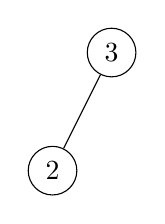
\begin{tikzpicture}
      \node[circle,draw](z){3}
        child {
          node[circle,draw]{2}
            child[missing]
            child[missing]
        }
        child[missing];
      \end{tikzpicture}
  \end{subfigure}%
  \begin{subfigure}{0.3\textwidth}
    \centering
    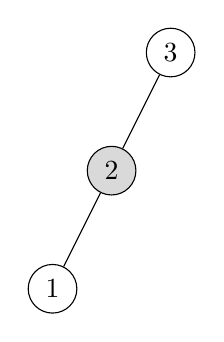
\begin{tikzpicture}
      \node[circle,draw](z){3}
        child {
          node[circle,draw,fill=gray!30]{2}
            child {
              node[circle,draw]{1}
                child[missing]
                child[missing]
            }
            child[missing]
        }
        child[missing];
      \end{tikzpicture}
  \end{subfigure}%
  \begin{subfigure}[c]{0.3\textwidth}
    \centering
    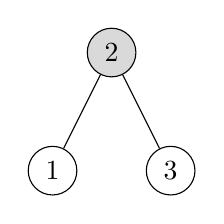
\begin{tikzpicture}
      \node[circle,draw,fill=gray!30](z){2}
        child{
          node[circle,draw]{1}
            child[missing]
            child[missing]
        }
        child{
          node[circle,draw]{3}
            child[missing]
            child[missing]
        };
    \end{tikzpicture}
  \end{subfigure}
  \caption{}
  \label{fig:rotation}
\end{figure}

An example of a simple right rotation is shown in Figure \ref{fig:rotation}. After the node with the key of 1 gets inserted, the tree becomes left-heavy, which can be fixed with a right rotation. The direct ancestor of the newly inserted node with the key of 2 becomes the new root of the tree, and the ancestor of the new root moves to the right. The result is a balanced tree, with order and the keys preserved.

\begin{lstlisting}
def simple_right : btree α → btree α
| btree.empty := btree.empty
| (btree.node (btree.node ll lk la lr) k a r) := 
    btree.node ll lk la (btree.node lr k a r)
| (btree.node l k a r) := btree.node l k a r
\end{lstlisting}

Compound rotations are performed when after a simple rotation the tree is still unbalanced. If after a left rotation, the tree is becomes left-heavy then a right rotation is done to fix the heaviness. The definition for \lstinline{rotate_left} is mirror. \todo{maybe add a figure here for compound rotations?}

\begin{lstlisting}
def rotate_right : btree α → btree α
| btree.empty := btree.empty
| (btree.node l k a r) :=
  match l with
  | btree.empty := (btree.node l k a r)
  | (btree.node ll lk la lr) :=
    if height ll < height lr 
      then simple_right (btree.node (simple_left l) k a r)
      else simple_right (btree.node l k a r)
  end 
\end{lstlisting}

The insertion definition makes use of the definitions of heaviness and rotations to insert a node into a tree while retaining balance. If insertion creates a left-heavy tree, then a right rotation is done, and if it creates a right-heavy tree, then a left rotation is done.

\begin{lstlisting}
def insert (x : nat) (v : α) : btree α → btree α
| btree.empty := btree.node btree.empty x v btree.empty
| (btree.node l k a r) :=
  if x < k then 
    if left_heavy (insert l) 
      then rotate_right (btree.node (insert l) k a r)
      else btree.node (insert l) k a r
  else if x > k then
    if right_heavy (insert r) 
      then rotate_left (btree.node l k a (insert r))
      else btree.node l k a (insert r)
  else btree.node l x v r
\end{lstlisting}  

Deleting a node is more complicated, and depends on the its children. If its left child is empty, then the node can be removed and replaced by its right child. If the left subtree is not empty, we need to \lstinline{shrink} it. The process of shrinking is simple -- we travel the tree recursively along its right subtrees, looking for a node whose right child is empty. During this process, if the tree becomes imbalanced a right rotation is completed. Once the node is found, the \lstinline{shrink} function returns its key, value, and the resulting shrunken tree. Since shrinking an empty tree is impossible, \lstinline{shrink} returns an \lstinline{option}.

\begin{lstlisting}[escapeinside={*}{*}]
  def shrink : btree α → option (nat × α × btree α)
  | btree.empty := none
  | (btree.node l k v r) := some *\$*
    match shrink r with
    | none := (k, v, l)
    | some (x, a, sh) :=
      if height l > height sh + 1
        then (x, a, rotate_right (btree.node l k v sh))
        else (x, a, btree.node l k v sh)
    end
  \end{lstlisting}

After defining shriking, the next step is to define the function \lstinline{del_node}. After the shrinking process is complete, a left rotation may be completed to re-balance the tree, and the key and node values of the tuple result of \lstinline{shrink} replace the key and value of the node to delete.

\begin{lstlisting}
def del_node : btree α → btree α
| btree.empty := btree.empty
| (btree.node l k v r) :=
  match shrink l with 
  | none := r
  | some (x, a, sh) :=
    if height r > height sh + 1 
      then rotate_left (node sh x a r)
      else node sh x a r
  end
\end{lstlisting}

Finally, the full \lstinline{delete} function is complete. 

\begin{lstlisting}
def delete (x : nat) : btree α → btree α
| btree.empty := btree.empty
| (btree.node l k a r) :=
  let dl := delete l in
  let dr := delete r in
  if x = k 
    then del_node (btree.node l k a r)
    else if x < k then
      if height r > height dl + 1 
        then rotate_left (btree.node dl k a r)
        else btree.node dl k a r
    else if height l > height dr + 1 then rotate_right (btree.node l k a dr)
    else (btree.node l k a dr)
\end{lstlisting}

First, find the node to delete. If it is found, then the \lstinline{del_node} function is called on the entire subtree. During the search of the node to delete, the operation is called recursively, and rotations are applied if the tree becomes unbalanced. 